\documentclass[titlepage]{article}

\usepackage{amsmath}
\usepackage{amsfonts}
\usepackage{amssymb}
\usepackage{graphicx}
\usepackage{float}
\usepackage{hyperref}
\usepackage{subfig}
\usepackage{url}
\usepackage{minted}
\usepackage[margin=0.75in]{geometry}
\graphicspath{{./assets/}}

\title{Exploring Fourier series from computational perspective}
\author{Igor Krzywda}

\begin{document}

\maketitle
\tableofcontents
\pagebreak

\section{Introduction}

    One time when I was binging YouTube, I stumbled upon a video by Grant Sanderson
    of 3Blue1Brown on Fourier series which featured many visualizations, prime of
    whose were drawings on a complex plain which were generated using Fourier
    series. Having done some reading on Fourier series as well as Fourier transform, 
    I decided that it would be a great idea to actually understand those concepts.
    Since for me the ultimate way of learning is solving problems and since I feel
    best at expressing ideas in code, I decided to set myself a challenge of 
    programming a program that will redraw my sketches with Fourier series.

\section{What is Fourier series?}

    The purpose of Fourier series is to approximate any periodic function with
    a sum of sines and cosines. The formula is given by~\eqref{eq:fs_rbase}
    \begin{equation} \label{eq:fs_rbase}
        S_\infty(t) = a_0 + \sum_{n=1}^{\infty}a_ncos\frac{2\pi nt}{P} + b_n%
            sin\frac{2\pi nt}{P}
    \end{equation}
    From the formula we can observe two things, each sine and cosine in the sum
    has a weight assigned to it ($a_n$ and $b_n$) and that $n$ determines the 
    frequency of the sinusoids. We can demistify the idea behind Fourier series
    by deriving formulas for all coefficients.

\subsection{Deriving $a_0$}
    
    First coefficient we will find is $a_0$, which is the only coefficient that 
    stands on its own. It is added before the actual series in order to compensate
    for the original function not oscillating around $x$ axis on the plot. It 
    basically is a vertical translation. We can see it if we add any constant
    to $sin(x)$, Figure~\ref{fig:sine_translation}.
    \begin{figure}[H]
        \caption{red : $sin(x)$, blue : $1 + sin(x)$}
        \centering
        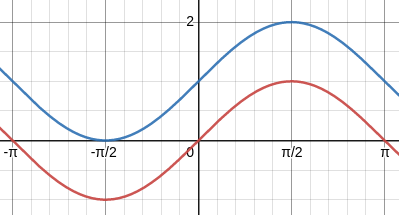
\includegraphics[width=0.5\linewidth]{translated_vanilla_sinewave}
        \label{fig:sine_translation}
    \end{figure}
    The problem to solve is to find the axis against which the sum will oscillate
    The solution to this problem is the average
    value of the original function over one period. The formula given for finding
    $a_0$ goes as follows~\eqref{eq:a0_formula}
    \begin{equation}\label{eq:a0_formula}
        a_0 = \frac{1}{P}\int_{\frac{P}{2}}^{\frac{-P}{2}}f(t)dt
    \end{equation}
    The average can be found through this formula because the 
    integral gives us the area under the graph of function $f(t)$ from 
    $-\frac{P}{2}$ to $\frac{P}{2}$. If we have an area, we can express it with 
    any figure that has this area, since we want an offset from the $x$ axis, 
    we can draw a rectangle whose base has length of $P$. Since we want to find
    out what the height of that rectangle is, we need to divide its area by its
    width, which is exactly what we are doing when dividing the integral by $P$.

\subsection{Finding $a_n$ and $b_n$}

    Coefficients $a_n$ and $b_n$ determine the amplitudes of sine waves of frequency
    $n$. Since the goal is to approximate some function $f(t)$ with a sum of 
    weighted sines and cosines, let that be the starting point.~\eqref{eq:eq_fs_f(t)}
    \begin{equation} \label{eq:eq_fs_f(t)}
        f(t) = a_0 + \sum_{n=1}^{\infty}a_ncos\frac{2\pi nt}{P} + b_n%
            sin\frac{2\pi nt}{P}
    \end{equation}
    In order to find the coefficients, we can exploit the properties of definite
    integrals of sine and cosine. To do that, we will need to expand the whole 
    expression by either $cos\frac{2\pi nt}{P}$ when looking for $a_n$, or by 
    $sin\frac{2\pi nt}{P}$ if we are looking for $b_n$. 

\subsubsection{Finding $a_n$}

    The expanded equation used to find $a_n$ looks like this~\eqref{eq:fs_exp_cos}.
    \begin{equation}\label{eq:fs_exp_cos}
    \begin{split}
        \int_{-\frac{P}{2}}^{\frac{P}{2}}f(t)cos\frac{2\pi nt}{P}dt 
        = \int_{-\frac{P}{2}}^{\frac{P}{2}}a_0cos\frac{2\pi nt}{P}dt 
        & +\int_{-\frac{P}{2}}^{\frac{P}{2}}a_1cos\frac{2\pi t}{P}cos\frac{2\pi nt}{P}dt +
        \int_{-\frac{P}{2}}^{\frac{P}{2}}b_1sin\frac{2\pi t}{P}cos\frac{2\pi nt}{P}dt \\
        & + \int_{-\frac{P}{2}}^{\frac{P}{2}}a_2cos\frac{4\pi t}{P}cos\frac{2\pi nt}{P}dt +
        \int_{-\frac{P}{2}}^{\frac{P}{2}}b_2sin\frac{4\pi t}{P}cos\frac{2\pi nt}{P}dt \\
        & \vdots \\
        & + \int_{-\frac{P}{2}}^{\frac{P}{2}}a_ncos^2(\frac{2\pi nt}{P})dt +
        \int_{-\frac{P}{2}}^{\frac{P}{2}}b_nsin\frac{2\pi nt}{P}cos\frac{2\pi nt}{P}dt 
        + ...
    \end{split}
    \end{equation}
    From this rather long expansion we can distill and solve for five cases appearing
    on the right side of the equation:
    \begin{enumerate}
        \item \begin{equation*}
                \int_{-\frac{P}{2}}^{\frac{P}{2}}a_0cos\frac{2\pi nt}{P}dt
                = a_0 \cdot \left[\frac{P}{2\pi n}sin\frac{2\pi nt}{P}\right]_{-\frac{P}{2}}^{\frac{P}{2}}
                = a_0 \cdot \frac{P}{2\pi n}(sin(\pi n) - sin(-\pi n)) = 0
              \end{equation*}
        \item For $m \in N$ and $m \neq n$
            \begin{equation*}
            \begin{split}
                \int_{-\frac{P}{2}}^{\frac{P}{2}} a_mcos \frac{2\pi mt}{P} 
                cos\frac{2\pi nt}{P} dt %
                %-------------------------------------------------------------
                & = a_m \cdot \int_{-\frac{P}{2}}^{\frac{P}{2}} \frac{1}{2} 
                \left( cos\frac{(m-n)2 \pi t}{P} 
                + cos\frac{(m+n)2 \pi t}{P} \right) dt \\%
                %-------------------------------------------------------------
                & = \frac{a_m}{2} \cdot \left[ \frac{P}{(m-n)2\pi n}
                sin\frac{(m-n)2 \pi t}{P} + \frac{P}{(m+n)2\pi n} 
                sin\frac{(m+n)2 \pi t}{P}  \right]_{-\frac{P}{2}}^{\frac{P}{2}} \\%
                %-------------------------------------------------------------
                & = \frac{Pa_m}{4\pi} \left( \frac{1}{m-n}sin((m-n)\pi)
                + \frac{1}{m+n} sin((m+n)\pi) \right. \\
                & \left. - \frac{1}{m-n} sin(-(m-n)\pi) - \frac{1}{m+n} 
                sin(-(m+n)\pi) \right) = 0
            \end{split}
            \end{equation*}
        \item For $m \in N$ and $m \neq n$
            \begin{equation*}
            \begin{split}
                \int_{-\frac{P}{2}}^{\frac{P}{2}} b_msin \frac{2\pi mt}{P} 
                cos\frac{2\pi nt}{P}dt %
                %-------------------------------------------------------------
                & = b_m \cdot \int_{-\frac{P}{2}}^{\frac{P}{2}}\frac{1}{2} 
                \left(sin\frac{(m+n)2 \pi t}{P} + 
                sin\frac{(m-n)2 \pi t}{P}\right)dt \\ %
                %-------------------------------------------------------------
                & = \frac{b_m}{2} \cdot \left[\frac{-P}{2\pi(m+n)}cos\frac{(m+n)2\pi t}{P}
                + \frac{-P}{2\pi(m-n)}cos\frac{(m-n)2\pi t}{P}
                \right]_{-\frac{P}{2}}^{\frac{P}{2}} \\ %
                %-------------------------------------------------------------
                & = \frac{Pb_m}{4\pi} \left( \frac{-1}{m+n}cos((m+n)\pi)
                + \frac{-1}{m-n} cos((m-n)\pi) \right. \\
                & \left. - \frac{-1}{m+n} cos(-(m+n)\pi) - \frac{-1}{m-n} 
                cos(-(m-n)\pi) \right) = 0
            \end{split}
            \end{equation*}
        \item 
            \begin{equation*}
            \begin{split}
                \int_{-\frac{P}{2}}^{\frac{P}{2}} b_nsin \frac{2\pi nt}{P} 
                cos\frac{2\pi nt}{P}dt %
                %-------------------------------------------------------------
                & = b_n \int_{-\frac{P}{2}}^{\frac{P}{2}} \frac{1}{2} \left
                sin\frac{4\pi nt}{P} + sin(0) \right) dt \\ %
                %-------------------------------------------------------------
                & = \frac{b_n}{2} \left[ \frac{-P}{4\pi n}cos\frac{4\pi nt}{P}
                - cos(0) \right]_{-\frac{P}{2}}^{\frac{P}{2}} \\ %
                %-------------------------------------------------------------
                & = \frac{b_n}{2} \left( \frac{-P}{4\pi n}cos(2\pi n) - 1 
                - \frac{-P}{4\pi n}cos(-2\pi n) + 1 \right) = 0
            \end{split}
            \end{equation*}
        \item
            \begin{equation*}
            \begin{split}
                \int_{-\frac{P}{2}}^{\frac{P}{2}}cos^2(\frac{2\pi nt}{P})dt
                & = \frac{1}{2}\int_{-\frac{P}{2}}^{\frac{P}{2}}1 + cos\frac{4\pi nt}{P}dt 
                = \frac{1}{2} \cdot \left[t + \frac{P}{4\pi n}sin\frac{4\pi nt}{P}
                \right]_{-\frac{P}{2}}^{\frac{P}{2}} \\
                & = \frac{1}{2}\left( \frac{P}{2} - \frac{4\pi n}{P}sin(2\pi n) + 
                \frac{P}{2} + \frac{4\pi n}{P}sin(-2\pi n)\right) = \frac{P}{2}
            \end{split}
            \end{equation*}
    \end{enumerate}

    We can see that the only term after expansion and integration that does not 
    amount to zero is $\int_{-\frac{P}{2}}^{\frac{P}{2}}cos^2(\frac{2\pi nt}{P})dt$,
    which means that our equation will simplify to the following form~\eqref{eq:fs_simp_cos}
    \begin{equation}\label{eq:fs_simp_cos}
        \int_{-\frac{P}{2}}^{\frac{P}{2}}f(t)cos\frac{2\pi nt}{P}dt = a_n\frac{P}{2}
    \end{equation}
    So in order to find $a_n$, we will get the following\eqref{eq:a_n}
    \begin{equation}\label{eq:a_n}
        a_n = \frac{2}{P}\int_{-\frac{P}{2}}^{\frac{P}{2}}f(t)cos\frac{2\pi nt}{P}dt
    \end{equation}
    Formula for $b_n$ is very similar~\eqref{eq:b_n} and stems from the same logic as one of 
    $a_n$, see Appendix A for calculations.
    \begin{equation}\label{eq:b_n}
        b_n = \frac{2}{P}\int_{-\frac{P}{2}}^{\frac{P}{2}}f(t)sin\frac{2\pi nt}{P}dt
    \end{equation}

\subsection{Even and odd functions in context of Fourier series}

    Last thing that will improve the efficiency with which coefficients can be
    computed is recognizing the fact whether the input function is an even or odd
    one. Even function can be described as $f(t) = f(-t)$ and an odd function can
    be described as $f(t) = -f(-t)$. This fact is important in integration, as there
    are formulas describing definite integrals of even and odd functions over an
    interval $[-a,a]$, which we are doing when computing the coefficients. The 
    definite integral for an even function $g(t)$ is in equation~\eqref{eq:int_even_func}.
    \begin{equation}\label{eq:int_even_func}
        \int_{-a}^{a}g(t)dt = 2\int_{-a}^{a}g(t)dt
    \end{equation}
    Definite integral for an odd function $h(t)$ is given in~\eqref{eq:int_odd_func}.
    \begin{equation}\label{eq:int_odd_func}
        \int_{-a}^{a}h(t)dt = 0
    \end{equation} 
    \\
    In context of Fourier series this is very useful, because if we look at sine
    and cosine functions, we can say that they are odd and even respectively:
    \begin{itemize}
        \item $sin(\theta) = -sin(-\theta)$
        \item $cos(\theta) = cos(-\theta)$ 
    \end{itemize}
    If the input
    function $f(t)$ is either even or odd, we need to pay attention to how
    the functions that describe $a_n$ and $b_n$ look like, because if this function
    is odd, we can establish from the start that is is zero. If both functions
    are the same in terms of being even or odd, then the product function will
    be even. If one function is even and other is odd, however, then the product
    function will be odd. Coming back to Fourier series, if we are computing 
    coefficients $a_n$ and $b_n$, we can state that:
    \begin{itemize}
        \item if function $f(t)$ is even, then
            \begin{equation*}
                b_n = \frac{2}{P}\int_{-\frac{P}{2}}^{\frac{P}{2}}f(t)sin\frac{2\pi nt}{P}dt = 0
            \end{equation*}
        \item if function $f(t)$ is odd, then
            \begin{equation*}
                a_n = \frac{2}{P}\int_{-\frac{P}{2}}^{\frac{P}{2}}f(t)cos\frac{2\pi nt}{P}dt = 0
            \end{equation*}
        \end{itemize}

\subsection{Approximating a step function}
    
    Before diving straight to other concepts and the drawings, let us 
    take a second and manually approximate a step function defined in ~\eqref{eq:step}
    and plotted in Figure~\ref{fig:step_func}

    \begin{equation}\label{eq:step}
    \begin{split}
         &f(t) = 
        \begin{cases} 
            & -2 \text{ if } -\pi \leq t < 0 \\
            & 2 \text{ if }  0 \leq t \leq \pi
        \end{cases} \\
        & f(t) = f(t + 2\pi) 
    \end{split}
    \end{equation}

    \begin{figure}[H]
        \caption{Step function f(t)}
        \centering
        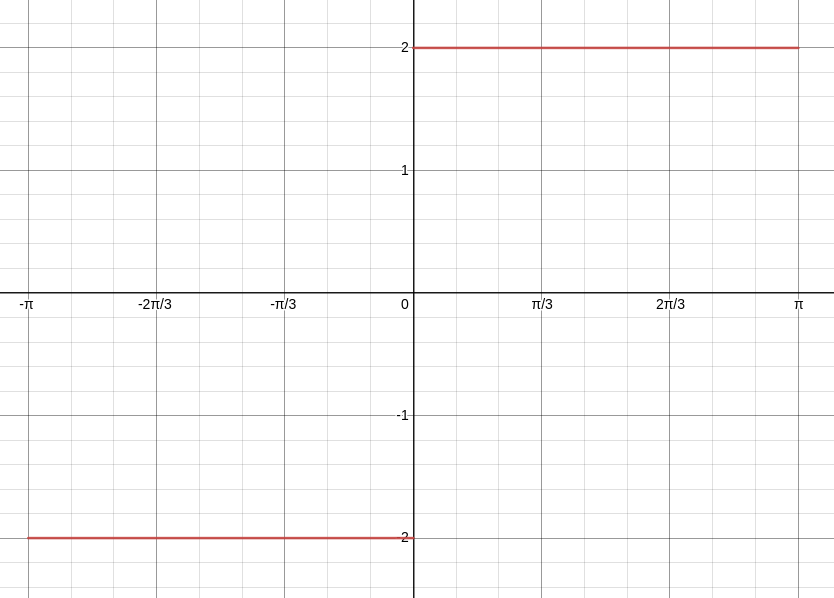
\includegraphics[width=0.5\linewidth]{step_func}
        \label{fig:step_func}
    \end{figure} 

    The function $f(t)$ is odd, so we only need to calculate coefficients $b_n$, as
    we know that all weights $a_n$ will amount to zero.

    \begin{equation}
    \begin{split}
        b_n & = \frac{2}{2\pi}\int_{-\pi}^{\pi}f(t)sin(nt)dt 
        = \frac{1}{\pi}\int_{-\pi}^{0}\frac{2}{n}cos(nt) + 
        \frac{1}{\pi}\int_{0}^{\pi}\frac{-2}{n}cos(nt) \\
        & = \frac{2}{\pi n}\left(\left[cos(nt) \right]_{-\pi}^{0}
        - \left[cos(nt) \right]_{0}^{\pi} \right) \\
        & = \frac{2}{\pi n}\left(cos(0) - cos(-n\pi) - cos(n\pi) + cos(0)\right) \\
        & = \frac{2}{\pi n}\left(2 - 2cos(n\pi)\right) 
        = \frac{4}{\pi n}\left(1 - cos(n\pi)\right) = 
        \begin{cases} 
            & \frac{8}{n\pi} \text{ if n is odd} \\
            & 0 \text{ if n is even}
        \end{cases} 
    \end{split}
    \end{equation}
    
    The series for our step function looks like this~\eqref{eq:step_fs}.
    \begin{equation}\label{eq:step_fs}
        S_\infty(t) = \sum_{n=1}^{\infty}\frac{8}{(2n-1)\pi}sin((2n - 1)t)
    \end{equation}

    Now we can make a few plots of the series with increasing number of terms
    and see it converge to $f(t)$, Figure~\ref{step_fs_plots}
    \begin{figure}[H]
    \caption{}
    \begin{tabular}{cc}
    \subfloat[n = 0]{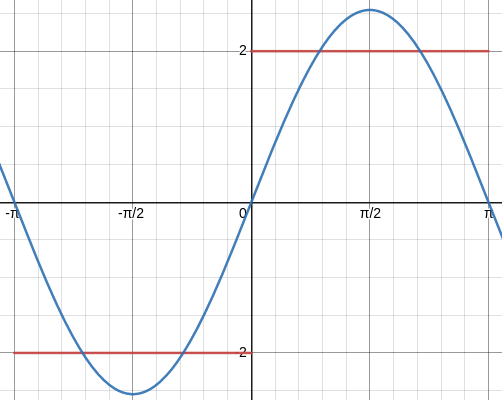
\includegraphics[width=0.4\linewidth]{step_approx_1}} &
    \subfloat[n = 2]{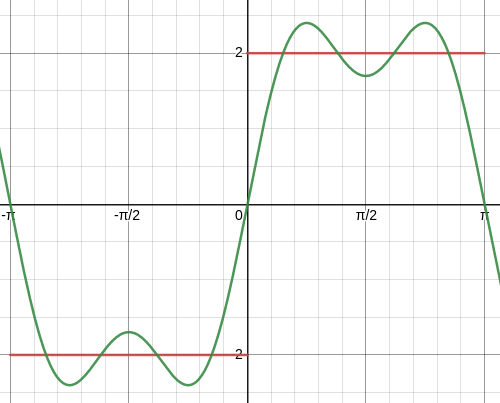
\includegraphics[width=0.4\linewidth]{step_approx_2}}\\
    \subfloat[n = 5]{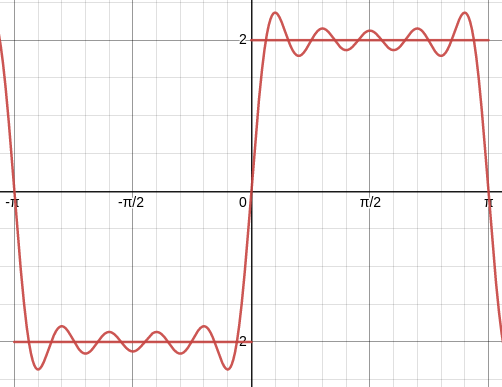
\includegraphics[width=0.4\linewidth]{step_approx_3}} &
    \subfloat[n = 7]{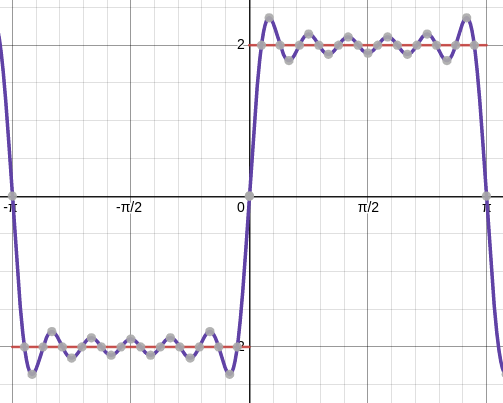
\includegraphics[width=0.4\linewidth]{step_approx_4}}
    \end{tabular}
    \label{step_fs_plots}
    \end{figure}

    In the plots above we can clearly see the convergence of the series to the
    function $f(t)$, however the series does not converge well to points at
    $-\pi$, $0$ and $\pi$, which shows that the approximations done with Fourier
    series are not fully precise.


\section{Overview of the program} 

\subsection{Taking input}
    
    Input is taken from the user in form of an array of $(X,Y)$ coordinates on 
    a window prompted using SFML (Simple and Fast Multimedia Library) for C++ 
    programming language (Figure~\ref{fig:input_window}). If the mouse is 
    left-clicked and moved, the coordinates
    are recorded and saved in the array, as well as printed on the window. 
    \begin{figure}[H]
        \caption{}
        \centering
        
\includegraphics[width=0.3\linewidth]{input_window}
        \label{fig:input_window}
    \end{figure}

\subsection{Implementation of complex numbers}

    The drawing is a set of points with $x$ and $y$ coordinates, however, all 
    calculations done in the next stages need to be done on complex numbers.
    Akin to points that are described in terms of coordinates, complex numbers
    are also described in terms of
    two dimensions. One of them everyone knows really well, because this is the 
    the real component, which, as the name suggests, consists of real numbers.
    The component that allows us to move vertically does not belong on the real 
    number line because this number is $\sqrt{-1}$, usually denoted as $i$. So
    any complex number can be denoted as following: $a + bi$ and can be depicted
    like in figure~\ref{fig:complex_number}
    \footnote{Graphic taken from \url{https://en.wikipedia.org/wiki/Complex_number}}
    \begin{figure}[H]
        \caption{}
        \centering
        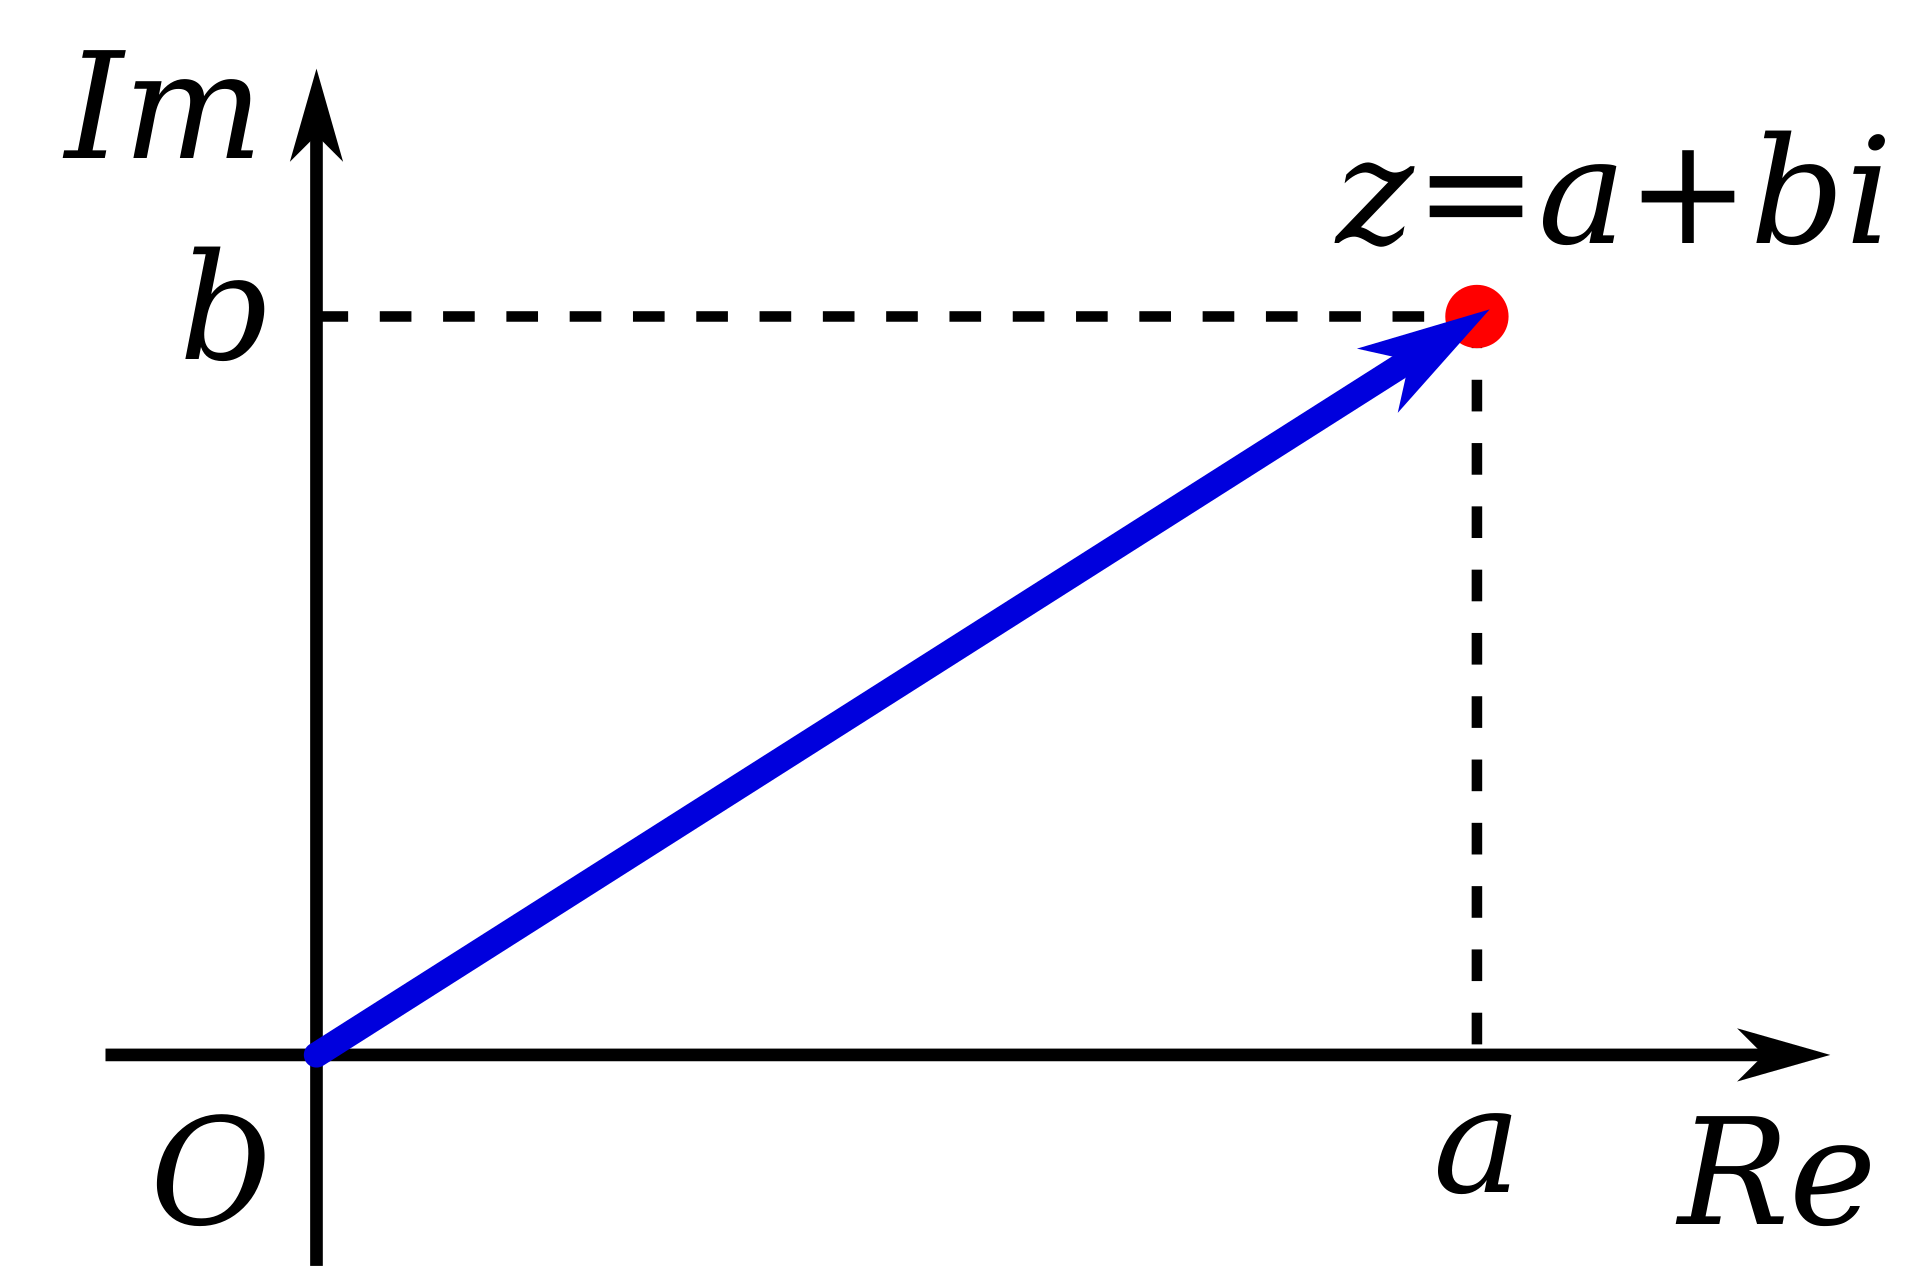
\includegraphics[width=0.3\linewidth]{imaginary_number}
        \label{fig:complex_number}
    \end{figure}
    The implementation of complex numbers in code is a template structure 
    containing two fields - real component (\texttt{re}) and imaginary (\texttt{im}).
    \begin{minted}{C++}
template <class T>
struct Complex
{
    T re = 0, 
      im = 0;
}
    \end{minted}
    The most important thing, however, is overloading operators for this structure,
    which will make later code much more readable. Below is an example of overloading
    multiplication operator that will be used a lot in later code. The implementation
    stems from equation~\eqref{eq:complex_mult}
    \begin{equation}\label{eq:complex_mult}
        (a + bi) \cdot (c + di) = ac - bd + adi + cbi 
    \end{equation}
    \begin{minted}{C++}
    Complex operator*(Complex n)
    {
        Complex t;

        t.re = this->re * n.re - this->im * n.im;
        t.im = this->re * n.im + this->im * n.re;

        *this = t;

        return *this;
    };
    \end{minted}

\subsection{Discrete Fourier transform (DFT)}

    Next step in the program is to find the coefficients for the Fourier series.
    However, the coefficients will be a bit different, since we are working with 
    a set of complex numbers rather than a function. This means that the series
    will have a different form, but first we need to find the weights, which can
    be found using DFT, which is defined by formula~\eqref{eq:dft_vanilla}.
    \begin{equation}\label{eq:dft_vanilla}
        X_k = \sum_{n=0}^{N-1}x_n \cdot \left[cos\left(\frac{2\pi}{N}kn\right) - 
        isin\left(\frac{2\pi}{N}kn\right)\right]
    \end{equation}
    Now let us walk through what each variable means:
    \begin{itemize}
        \item $X_k$ - output complex number of DFT
        \item $N$ - size of input set
        \item $k$ - frequency
        \item $x_n$ - $n^{th}$ complex number in the input set $\left\{x_0, x_1,
            ..., x_{N-1} \right\}$
    \end{itemize}
    
    The first thing to go through is why we are multiplying our input complex 
    number by a complex sum?

\subsubsection{Expressing a point on a unit circle using complex numbers}

    Let us take a right triangle with hypotenuse of length $1$
    (Figure~\ref{fig:right_triangle})
    and angle $\theta$ between that hypotenuse ($c$) and the base ($b$) of triangle.
    \begin{figure}[H]
        \caption{}
        \centering
        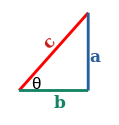
\includegraphics[width=0.2\linewidth]{right_triangle}
        \label{fig:right_triangle}
    \end{figure}
    If we wanted to find the length of the base ($b$), it would be equal
    to the $cos\theta$ since the hypotenuse has the length $1$. Similarly, if we
    wanted to find the height of the triangle ($a$), it would be the $sin\theta$.

    Now we can inscribe such right triangle into a unit circle on a complex plane
    where the hypotenuse of the triangle would simultaneusly be the radius of 
    the circle (Figure~\ref{fig:inscribed_triangle}) at angle $\theta$ between
    radius and the horizontal axis.
    \begin{figure}[H]
        \caption{}
        \centering
        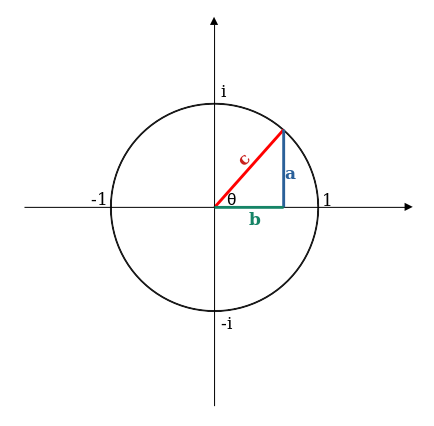
\includegraphics[width=0.4\linewidth]{inscribed_triangle}
        \label{fig:inscribed_triangle}
    \end{figure}
    We can find the complex value for the point where the radius touches the circumference
    using the inscribed triangle, so $cos\theta$ would be the horizontal coordinate
    and $i \cdot sin\theta$ would be the vertical component since we are on complex
    plane. So the whole position can be described as $cos\theta + isin\theta$.
    Conversly, if $cos\theta + isin\theta$ are plotted for every $\theta$ between
    $0$ and $2\pi$, we get an unit circle on a complex plane.


\subsubsection{Applying Discrete Fourier Transform}
    
    The formula for DFT is a sum, however in order to visualize what is happening
    when applying DFT to a set of values, we will plot all values that are being
    summed, as well as the average of this sum (an average is taken normally when
    applying Fourier series, however, it can also be done during DFT, which will
    aid the readibility of the plots).
    Let us apply Discrete Fourier Transform to an easy-to-
    visualize example. We will plot all results from expression~\eqref{eq:mapping}
    \begin{equation}\label{eq:mapping}
        x_n \cdot \left[cos\left(\frac{2\pi}{N}kn\right) - isin\left(
            \frac{2\pi}{N}kn\right)\right]
    \end{equation}
    where $x_n$ are the elements of set, which is a discrete
    form of $cos(2\theta)$ from $0$ to $2\pi$, and $k$ (or frequency) is $1$, which 
    means that all values will be mapped within one revolution around the unit circle
    (Figure~\ref{fig:cos_wrapped}, where subfigure~\ref{subfig:cos_2t} is the plot
    of set $x$ and subfigure~\ref{subfig:cos_2t_wrapped} is the plot of results)
    of the expression~\eqref{eq:mapping}
    \begin{figure}[H]
      \caption{}\label{fig:cos_wrapped}
      \centering
        \subfloat[$cos(2t)$]{%
            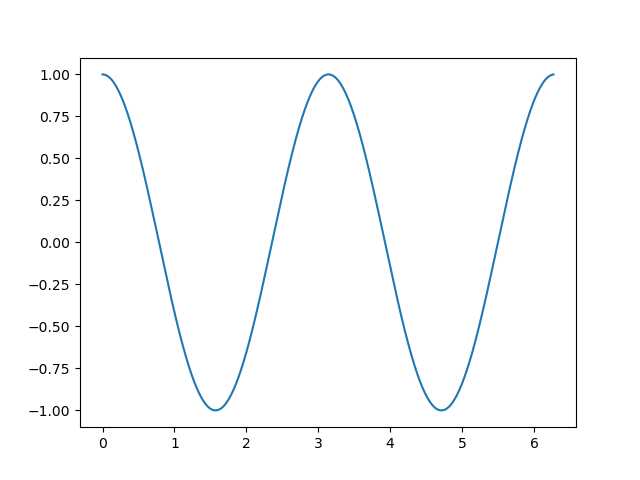
\includegraphics[width=0.4\textwidth]{cos_vanilla}%
            \label{subfig:cos_2t}%
            }
      \hfill
        \subfloat[$cos(2t)$ - wrapped]%
            {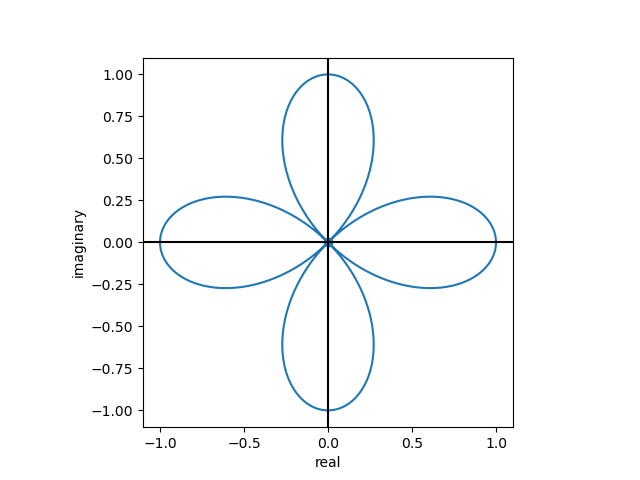
\includegraphics[width=0.4\textwidth]{cos_wrapped}%
            \label{subfig:cos_2t_wrapped}%
            }
    \end{figure}
    In plot~\ref{subfig:cos_2t_wrapped} we can see that the values have aligned
    in a shape that is symmetric about real (horizontal) and imaginary (vertical)
    axes, which means for every element in the set, there is another one, which
    has an inverse value, which, after summing all values gives zero. 


    If we do the same operation, but now we change $k$ to match the frequency of
    the input, which is $2$, as the function $cos(2t)$, that the input set is a discrete
    form of, completes two cycles in one period. If we plot all of those values
    along with the average of the sum, we get what is shown in 
    Figure~\ref{fig:cos_wrapped_2k}.
    \begin{figure}[H]
        \caption{}
        \centering
        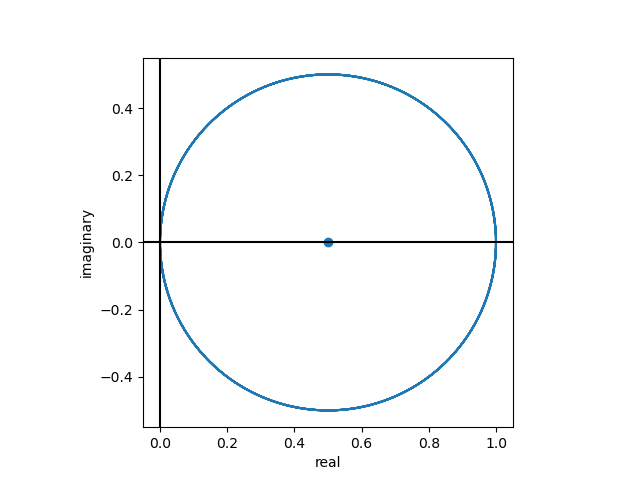
\includegraphics[width=0.4\linewidth]{cos_wrapped_2k}
        \label{fig:cos_wrapped_2k}
    \end{figure}
    The shape that the values formed in this case is different, as it is only 
    symmetric horizontally, which means that the imaginary components will cancel
    out, whereas the real components will give a non-zero value, which, after
    taking the average is in the center of this shape.


    The results of DFT tell how much present a component that can be described as
    $cos\left(\frac{2\pi}{N}kn\right) - isin\left( \frac{2\pi}{N}kn\right)$ is 
    in the set. The concrete values are used later on in phase where Fourier 
    series is used.


    We can, however, take a look how the values will align when we will be applying
    DFT to sets that are a discrete form of sum of sinusoids. This is one of the 
    most important uses of DFT, as sound signals are composed of many sine waves 
    with different frequencies and DFT allows for finding those frequencies. 
    As an example we shall take a function $f(t) = cos(10t) + cos(20t) + sin(25t)$, 
    whose plot is shown in Figure~\ref{fig:composed}. We can expect non-zero 
    values for $k = {10,20,25}$.

    \begin{figure}[H]
        \caption{}
        \centering
        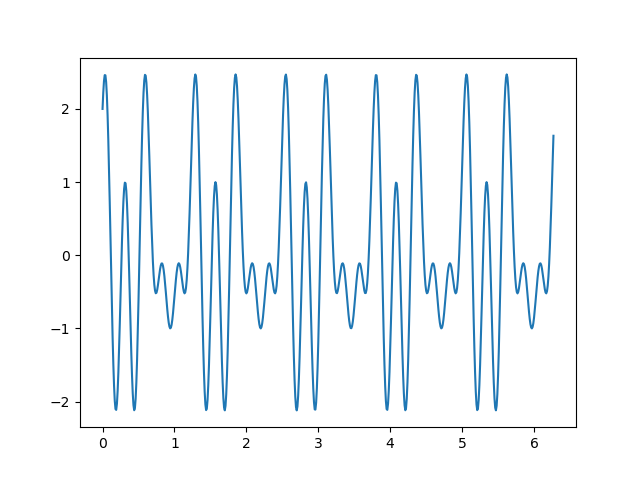
\includegraphics[width=0.4\linewidth]{composed}
        \label{fig:composed}
    \end{figure}
    Below, in Figure\ref{fig:step_fs_plots} we can see the plots of all elements
    of input set multiplied by $cos\left(\frac{2\pi}{N}kn\right) - isin\left( 
    \frac{2\pi}{N}kn\right)$. $k$ in the
    captions shows the value of $k$ used in the expression and the dots in the
    plots are the averages of the results of DFT.
    $\frac{1}{N}$
    \begin{figure}[H]
    \caption{}
    \begin{tabular}{cc}
    \subfloat[k = 1]{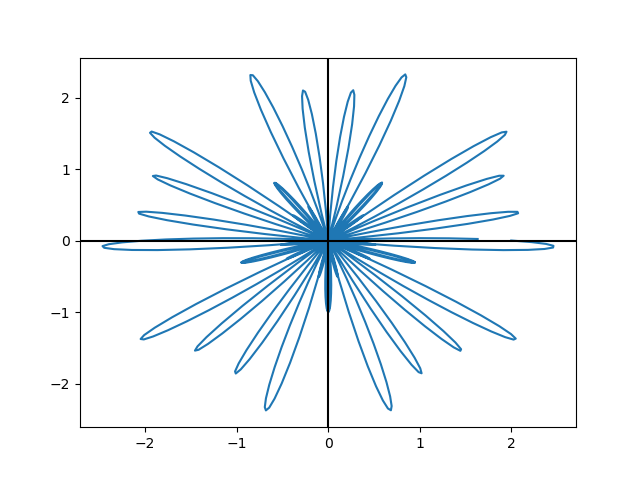
\includegraphics[width=0.4\linewidth]{composed_wrapped}} &
    \subfloat[k = 10]{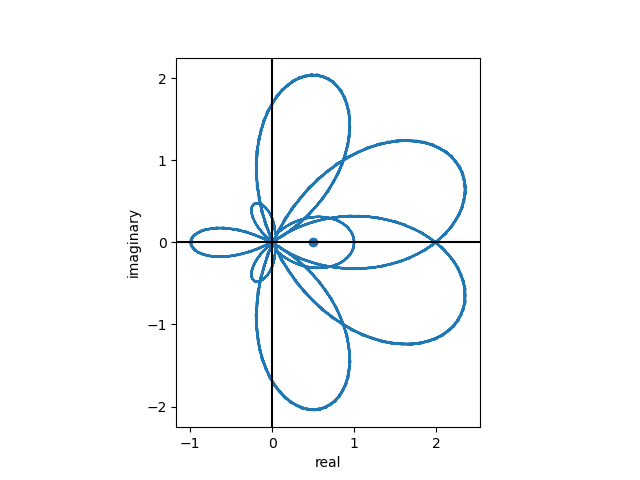
\includegraphics[width=0.4\linewidth]{decomposed_1}}\\
    \subfloat[k = 20]{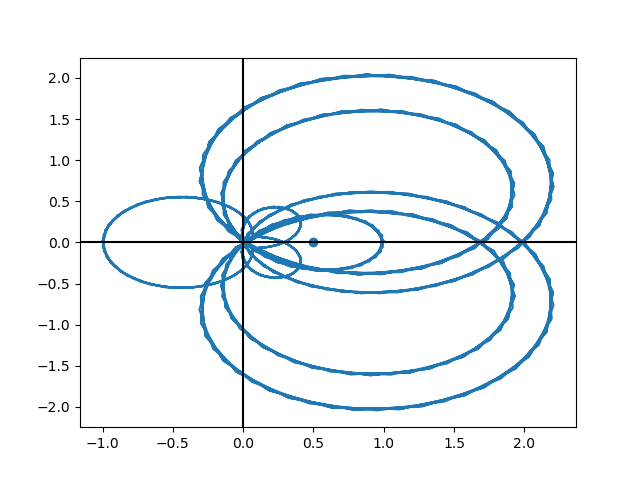
\includegraphics[width=0.4\linewidth]{decomposed_2}} &
    \subfloat[k = 25]{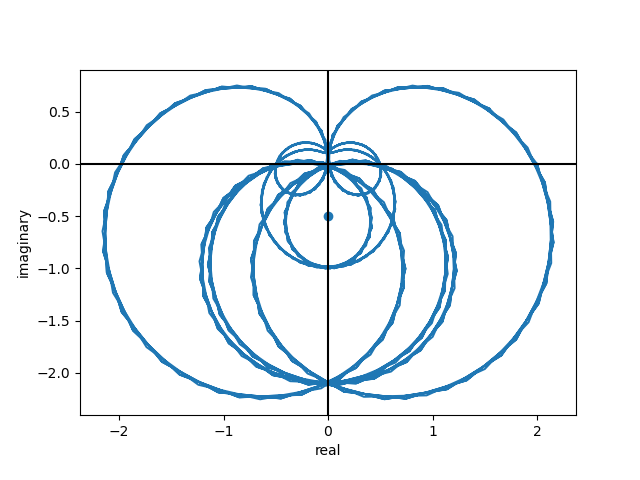
\includegraphics[width=0.4\linewidth]{decomposed_3}}
    \end{tabular}
    \label{step_fs_plots}
    \end{figure}
    We can see that for values of $k$ that correspond to the frequencies of the
    sinusoids making up the original function, the plots bias towards one side,
    which causes the sums of all those values to be bigger than zero.
    
    See Appendix B for source code of script used to generate all plots above.

\subsubsection{Why naive implementation of DFT is inefficient}

    Below is implementation of DFT that is inside the source code of the program.

    \begin{minted}{C++}

C_set *DFT(C_set input)
{
    C_set *out = new C_set;
    C temp, X_k;
    unsigned N = input.size();
    double a = (2 * M_PI) / N, x;

    for (unsigned k = 0; k < N; ++k)
    {
        for (unsigned n = 0; n < N; ++n)
        {
            x = a * n * k;
            temp = C(cos(x), -sin(x));

            X_k += (temp * input[n]);
        }

        out->push_back(X_k);
        X_k = C(0,0);
    }

    return out;
}
    \end{minted}

    Inside the function there are two for loops. The first one iterates through
    frequencies ($k$) as we want more coefficients than for one frequency. The 
    inner loop is the exact implementation of the formula for DFT, where all terms
    from the input set are multiplied by $cos\left(\frac{2\pi}{N}kn\right) - isin\left( 
    \frac{2\pi}{N}kn\right)$ and added together to compute the coefficient for 
    frequency $k$. This is also the source of the inefficiency of this algorithm.
    Because there are two nested loops that go from $0$ to $N-1$, the time complexity
    of this algorithm is $\mathcal{O}(n^2)$, which means that given an input of 
    size $n$, the computer will make $n^2$ operations. This is very inefficient
    and slow for real-life applications of DFT, as the sizes of inputs for those
    applications can get very big. For example, a WAV file containing 1 second of
    audio signal has $44'100$ samples. Processing a short song would take a lot
    of computing resources. This is why in most actual implementations of DFT,
    an algorithm called Fast Fourier Transform (FFT) is used, whose time complexity
    is $\mathcal{O}(n\log(n))$.

\subsection{Fourier series and making drawings}

    The last stage of the program is to recreate the original drawing using the
    inverse discrete Fourier transform (IDFT), which is the same as discrete
    Fourier series\footnote{terms IDFT and discrete Fourier series will be used
    interchangeably in this section}. The formula is given in equation~\eqref{eq:IDFT}.
    \begin{equation}\label{eq:IDFT}
        x_n = \frac{1}{N}\sum_{k=0}^{N-1}X_k \cdot \left[cos\left(\frac{2\pi}{N}kn\right) +
        isin\left(\frac{2\pi}{N}kn\right)\right]
    \end{equation}
    In discrete Fourier series, the means of coefficients acquired through DFT 
    ($\frac{1}{N}X_k$) are used like weights $a_0$, $a_n$ and $b_n$ in case of 
    real form of Fourier series discussed in section 2. We already know that 
    expression $cos\theta + isin\theta$ returns complex value that represents a
    position at angle $\theta$ on a unit circle on a complex plane. The mean of
    the coefficient $X_k$ regulates the radius and phase of such circle. In figure
    ~\ref{fig:dfs_explainer_1}, there is one such circle multiplied by $3+4i$. We can
    see that the radius of this circle is the hypotenuse of right triangle formed
    by real and imaginary component of the complex number. Angle $\theta$ on the
    plot is the phase shift caused by the term $3+4i$, which we can think of as
    the point from which the circle is drawn. Now, even though we are 
    dealing with discrete values in IDFT, the values will ``rotate''
    as $n$ increases - Figure~\ref{fig:dfs_explainer_2}. Additionally, each term 
    has its $k$, which is the frequency, in this case meaning that values ``rotate''
    $k$ times within one period.
    \begin{figure}[H]
      \caption{}\label{fig}
      \centering
        \subfloat[]{%
            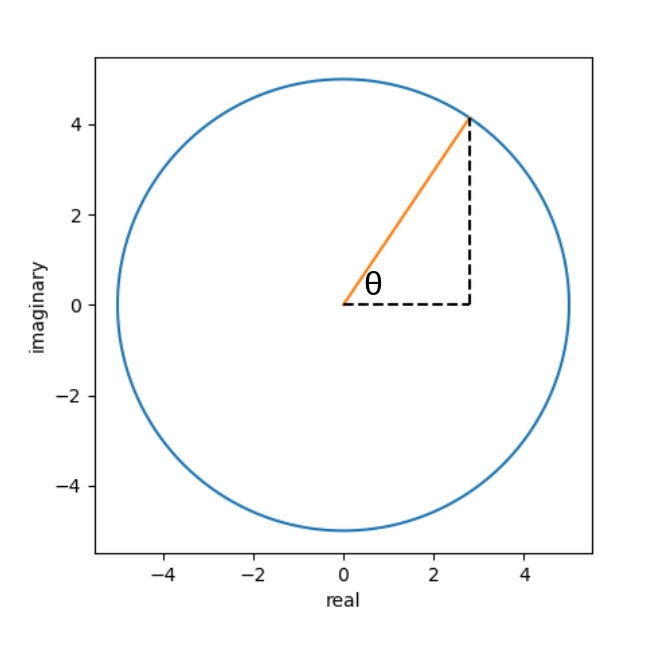
\includegraphics[width=0.4\linewidth]{dfs_explainer_1}%
            \label{fig:dfs_explainer_1}%
            }
      \hfill
        \subfloat[]%
            {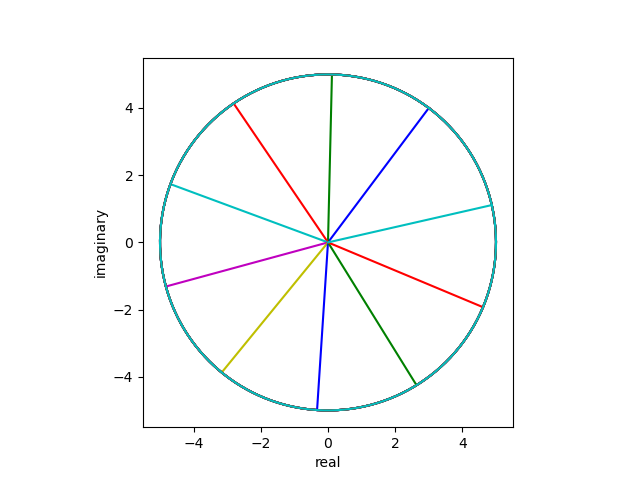
\includegraphics[width=0.5\linewidth]{dfs_explainer_2}%
            \label{fig:dfs_explainer_2}%
            }
    \end{figure}
    Because complex numbers are being added in the series, a good way to visualize
    this operation is by seeing complex numbers as lines that are ``attached'' together
    by their ends like in Figure~\ref{fig:complex_sum}. Then, in the context of 
    IDFT, we can think that each of those lines ``rotate'' by $\frac{2\pi}{N}k$ as we 
    compute the next term - Figure~\ref{fig:dfs_explainer_3}. 
    \begin{figure}[H]
      \caption{}\label{f}
      \centering
        \subfloat[]{%
            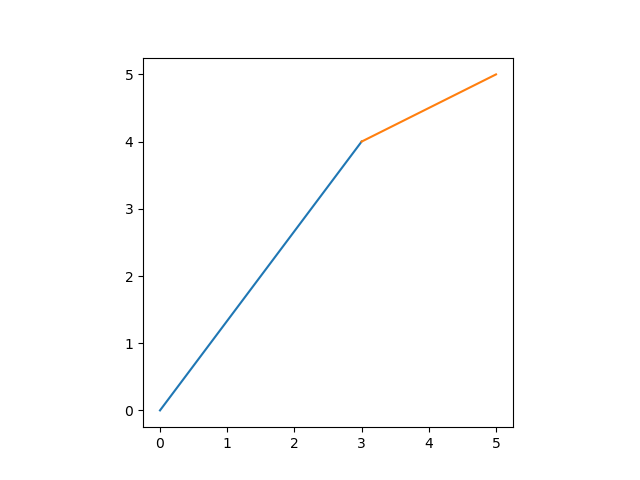
\includegraphics[width=0.5\linewidth]{complex_sum}%
            \label{fig:complex_sum}%
            }
      \hfill
        \subfloat[]%
            {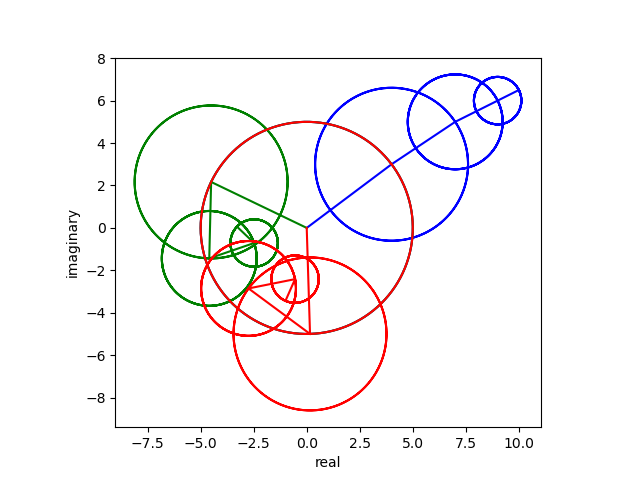
\includegraphics[width=0.5\linewidth]{dfs_explainer_3}%
            \label{fig:dfs_explainer_3}%
            }
    \end{figure}
    Since the plot is merely a representation of all terms summed in the series,
    the output value $x_n$ is at the end of each of collection of lines representing
    complex numbers. If we now plot the values returned by discrete Fourier 
    series with the same coefficients (Figure~\ref{fig:dfs_explainer_4}), we can 
    see some shape - and such shapes will be the drawings generated by the 
    program.
    \begin{figure}[H]
        \caption{}
        \centering
        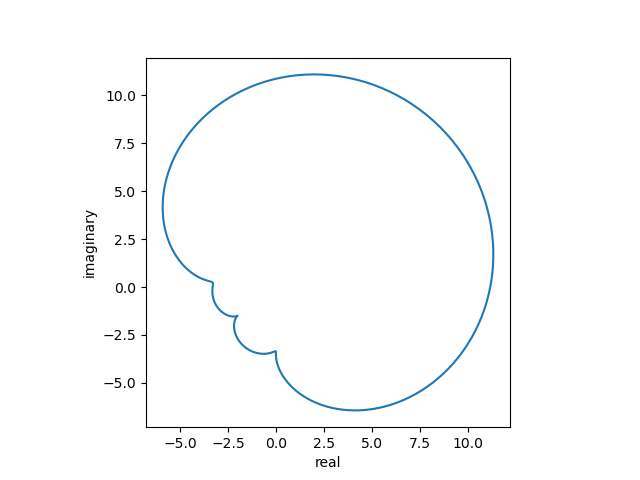
\includegraphics[width=0.5\linewidth]{dfs_explainer_4}
        \label{fig:dfs_explainer_4}
    \end{figure}
    One last thing to point out is that, like in case of real form of Fourier
    series, the more terms we add, the closer the ouptut will converge to the 
    input. So what the program does to visualize this convergence is it simply
    regulates the number of terms in the series, however this will be presented
    in the renders from the program.
    \paragraph{See Appendix C for the script used to generate all plots in the 
    section}

\subsubsection{Implementation of IDFT in code}

    Below is an implementation of IDFT in the source code of the program.
    \begin{minted}{C++}
void draw_IDFT(C_set &x_k, VertexArray &drawing, unsigned n)
{
    C temp, x_n;
    unsigned N = x_k.size();
    double step = (2 * M_PI) / N, theta;

    for (unsigned t = 0; t < N; ++t)
    {
        for (unsigned k = 0; k < n; ++k)
        {
            theta = step * t * k;     
            temp = C(cos(theta), sin(theta));

            x_n += (temp * x_k[k]) / N;
        }

        drawing[t] = Vector2f(x_n.re + 400, -x_n.im + 400);
        x_n = C(0,0);
    }
}
    \end{minted}

    The function takes a set of coefficients computed by DFT function (\texttt{x\_k}),
    an array of coordinates to be put on the screen (\texttt{drawing}) and a variable
    \texttt{n}, which allows for controlling how many terms are being added in the 
    series. The upper for loop iterates over one period in $N-1$ steps in order
    to get coordinates for a full period. The inner loop iterates from $0$ to $n$
    so that the user can regulate the number of arguments being added in the series
    and inside this loop is a direct implementation of IDFT. At the bottom, the 
    complex number \texttt{x\_n} is converted to coordinates that work with SFML 
    and is saved to the \texttt{drawing} array. 
    \paragraph{See Appendix D for instructions to compile the program on UNIX
    machine}

\section{Drawings}

    Below are sample examples of the program working. A few frames from the 
    program have been picked in order to best depict the working of both program
    and discrete Fourier series. $N$ in the top-left corner is the size of set
    containing DFT coefficients.

\subsection{Triangle}

    \begin{figure}[H]
    \centering
    \caption{}
    \begin{tabular}{ccc}
    \subfloat[original input]{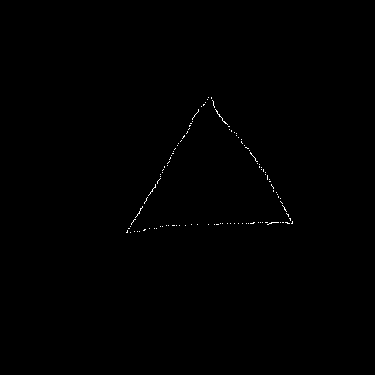
\includegraphics[width=0.3\linewidth]{fd_triangle_input}}\label{fig:triangles_1} &
    \subfloat[k = 2]{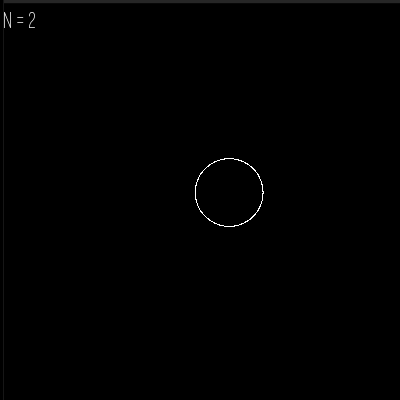
\includegraphics[width=0.3\linewidth]{fd_triangle_1}}\label{fig:triangles_2} &
    \subfloat[k = 15]{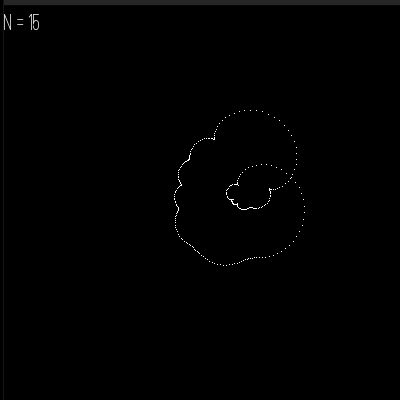
\includegraphics[width=0.3\linewidth]{fd_triangle_2}}\label{fig:triangles_3}\\
    \subfloat[k = 239]{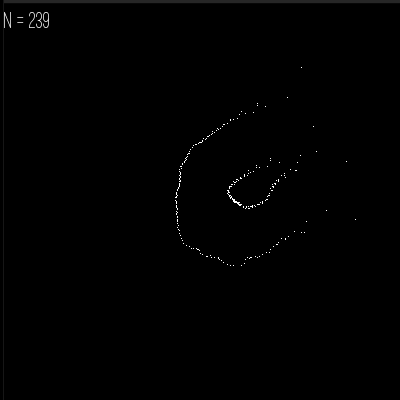
\includegraphics[width=0.3\linewidth]{fd_triangle_3}}\label{fig:triangles_4} &
    \subfloat[k = 314]{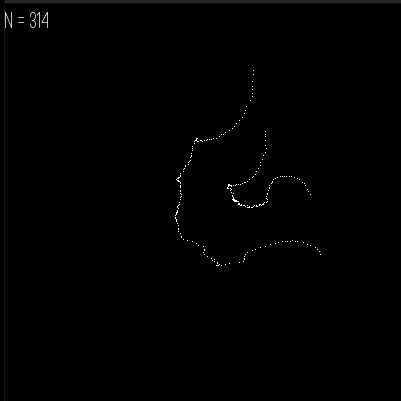
\includegraphics[width=0.3\linewidth]{fd_triangle_4}}\label{fig:triangles_5} &
    \subfloat[k = 322]{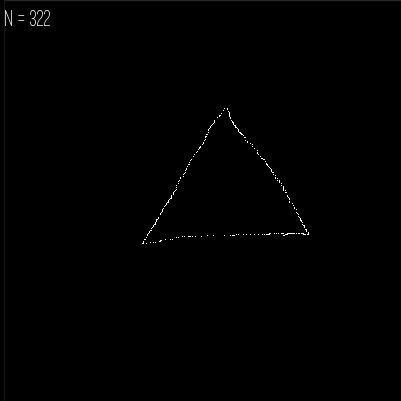
\includegraphics[width=0.3\linewidth]{fd_triangle_6}}\label{fig:triangles_6} 
    \end{tabular}
    \label{fig:triangles}
    \end{figure}
    
\subsection{Cube}

    \begin{figure}[H]
    \centering
    \caption{}
    \begin{tabular}{ccc}
    \subfloat[original input]{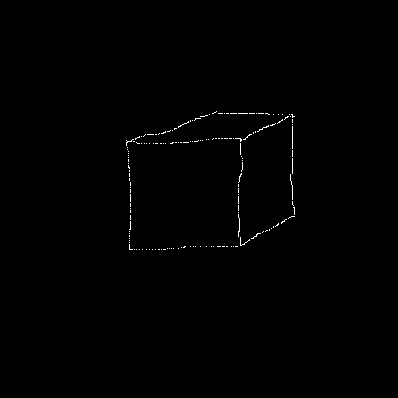
\includegraphics[width=0.3\linewidth]{fd_cube_input}} &
    \subfloat[k = 2]{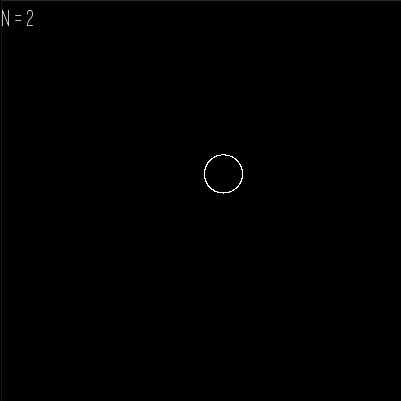
\includegraphics[width=0.3\linewidth]{fd_cube_1}} &
    \subfloat[k = 10]{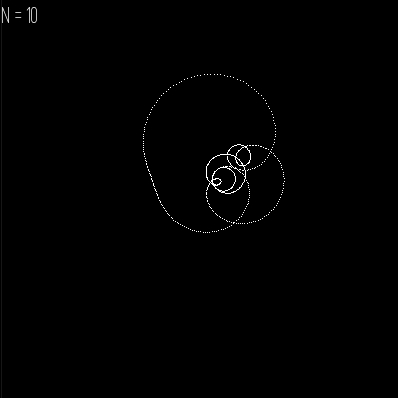
\includegraphics[width=0.3\linewidth]{fd_cube_2}}\\
    \subfloat[k = 403]{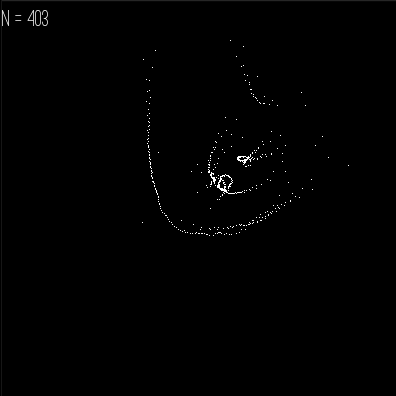
\includegraphics[width=0.3\linewidth]{fd_cube_3}} &
    \subfloat[k = 671]{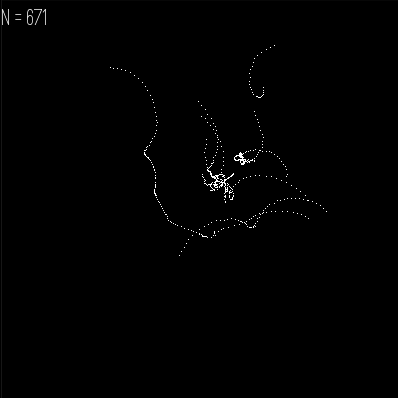
\includegraphics[width=0.3\linewidth]{fd_cube_4}} &
    \subfloat[k = 691]{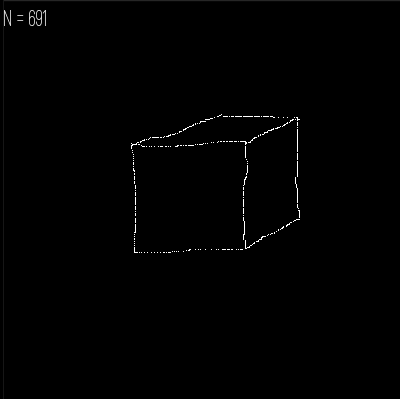
\includegraphics[width=0.3\linewidth]{fd_cube_6}} 
    \end{tabular}
    \label{fig:cubes}
    \end{figure}

\subsection{Pi}

    \begin{figure}[H]
    \centering
    \caption{}
    \begin{tabular}{ccc}
    \subfloat[original input]{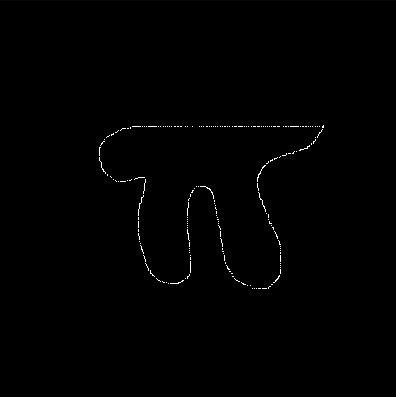
\includegraphics[width=0.3\linewidth]{fd_pi_input}} &
    \subfloat[k = 2]{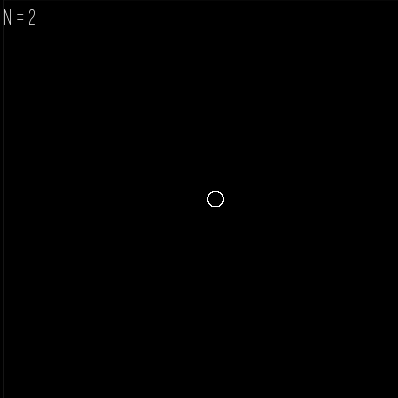
\includegraphics[width=0.3\linewidth]{fd_pi_1}} &
    \subfloat[k = 20]{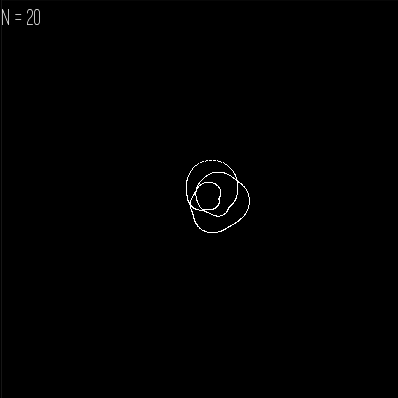
\includegraphics[width=0.3\linewidth]{fd_pi_2}}\\
    \subfloat[k = 710]{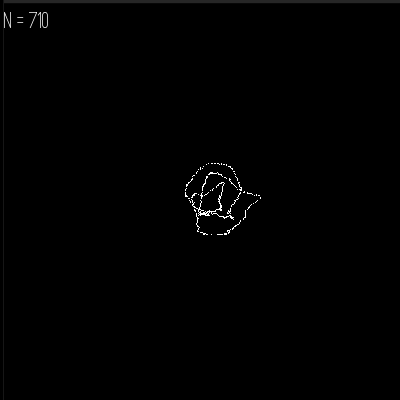
\includegraphics[width=0.3\linewidth]{fd_pi_3}} &
    \subfloat[k = 713]{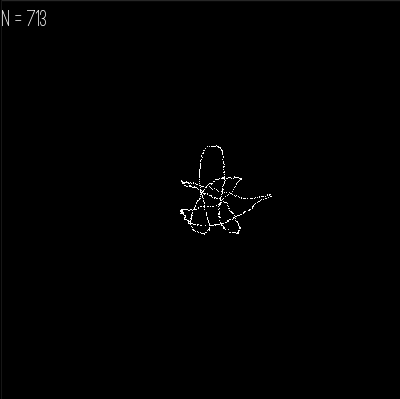
\includegraphics[width=0.3\linewidth]{fd_pi_4}} &
    \subfloat[k = 716]{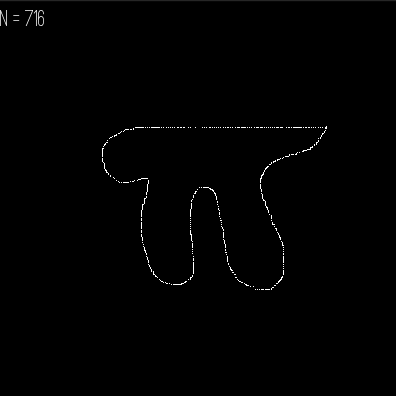
\includegraphics[width=0.3\linewidth]{fd_pi_6}} 
    \end{tabular}
    \label{fig:pis}
    \end{figure}

\section{Appendices}

\subsection{Appendix A}

\subsection{Appendix B}

    Python script used to depict workings of DFT.

    \begin{minted}{Python}
def wrap_function(func_in, freq):

    N = len(func_in)
    data = np.zeros(N, dtype = np.complex_)
    theta = (6.28 / N) * freq
    coeff = complex(0,0)

    for n in range(0, N):
        c = complex(m.cos(theta * n), -(m.sin(theta * n)))
        data[n] = func_in[n] * c
        coeff += data[n]

    coeff /= N

    return (data, coeff)


def plot_complex(data, name):

    plt.plot(data[0].real, data[0].imag)
    plt.scatter(data[1].real, data[1].imag)
    plt.axhline(y=0, color='k')
    plt.axvline(x=0, color='k')
    plt.savefig(sys.argv[1])

    plt.show()
    \end{minted}

    Modules needed to run the script:
    \begin{itemize}
        \item numpy
        \item matplotlib
        \item math
    \end{itemize}

\subsection{Appendix C}

    Python script used to generate data for plots used in explaining IDFT.

    \begin{minted}{Python}
def generate_fs(coeff, freq, offset):
    
    fs = np.fromfunction(
            np.vectorize(lambda i : 
                complex(np.cos((i * freq) / 100), 
                    np.sin((i * freq) / 100)) * coeff + offset),
            (629,), 
            dtype=complex)

    return fs
    \end{minted}

    Python script used to plot data.

    \begin{minted}{Python}
def plot_fs(coeff, epicycles, n, step):

    colors = ['b','g','r','c','m','y']

    if epicycles: 
        for k in range(n):
            offset = complex(0,0)
            fs = list()

            for i in range(0, len(coeff)):
                fs.append(generate_fs(coeff[i], i+1, offset))
                offset += (fs[i][k * step] - offset)

            offset = complex(0,0)

            for f in fs:
                color = colors[k % len(colors)]
                plt.plot(f.real, f.imag, color)
                plt.plot([offset.real,f[k * step].real], [offset.imag,f[k * step].imag], color)
                offset += (f[k * step] - offset)
    else:
        fs = list()
        for i in range(0, len(coeff)):
            fs.append(generate_fs(coeff[i], i+1, 0))
        out = sum(fs)
        plt.plot(out.real, out.imag)
        

    plt.gca().set_aspect('equal', adjustable='box')
    plt.xlabel('real')
    plt.ylabel('imaginary')
    plt.show()
    plt.savefig('dfs_explainer.png')

    \end{minted}

\subsection{Appendix D}

    \paragraph{Prerequisites}
    \begin{itemize}
        \item gcc / Clang / LLVM compiler for C++11 and higher
        \item SFML media library
    \end{itemize}

    \paragraph{Compilation and use guide for Fourier drawer program for UNIX machines:}
    \begin{enumerate}
        \item Clone git repository to your machine from the link:
            \url{https://github.com/ikrzywda/fourier\_drawer}
        \item change directory to \texttt{fourier\_drawer/drawer}
        \item use \texttt{make} to compile the program
        \item type \texttt{./fourier\_drawer} inside \texttt{drawer} directory to launch
            the program
    \end{enumerate}

    \paragraph{Controls}
    \begin{itemize}
        \item \textbf{left mouse button} to draw inside Fourier sketchpad window
        \item \textbf{Enter} to accept input given in Fourier sketchpad window
            and to terminate the program when in Fourier drawer window
        \item \textbf{K} to increase the number of arguments in Fourier drawer 
            window
        \item \textbf{J} to decrease the number of arguments in Fourier drawer 
            window
    \end{itemize}

\section{Bibliography}

    \begin{itemize}
        \item ``But what is the Fourier Transform? A visual introduction.'' YouTube, 
            uploaded by 3Blue1Brown, \url{https://www.youtube.com/watch?v=spUNpyF58BY}
        \item ``But what is a Fourier series? From heat flow to circle drawings | DE4'' 
            YouTube, uploaded by 3Blue1Brown, \url{https://www.youtube.com/watch?v=r6sGWTCMz2k}
        \item ``Electrical engineering : Signals and systems : Fourier series'' Khan
            Academy, \url{https://www.khanacademy.org/science/electrical-engineering/ee-signals#ee-fourier-series} 
        \item ``Discrete Fourier transform'', Wikipedia, \url{https://en.wikipedia.org/wiki/Discrete_Fourier_transform}
    \end{itemize}

\end{document}
